\appendix

\section{Metrics} \label{app:metric}
The evaluation for detection and tracking follows standard evaluation protocols\cite{nuscenes}. For detection, we use mean Average Precision(\textbf{mAP}), mean Average Error of
Translation(\textbf{mATE}), Scale(\textbf{mASE}), Orientation(\textbf{mAOE}), Velocity(\textbf{mAVE}), Attribute(\textbf{mAAE}) and nuScenes Detection Score(\textbf{NDS}) to evaluate the model performance. For tracking, we use Average Multi-object Tracking Accuracy(\textbf{AMOTA}), Average Multi-object Tracking Precision(\textbf{AMOTP}), \textbf{RECALL}, and Identity Switches(\textbf{IDS}) as the metrics. For online mapping, we calculate the Average Precision(\textbf{AP}) of three map classes: lane divider, pedestrian crossing and road boundary, then average across all classes to get mean Average Precision(\textbf{mAP}). For motion prediction, we employ metrics including minimum Average Displacement Error(\textbf{minADE}), minimum Final Displacement Error(\textbf{minFDE}), Miss Rate(\textbf{MR}) and End-to-end Prediction Accuracy(\textbf{EPA}) proposed in \cite{vip3d}. The motion prediction benchmark is aligned with UniAD\cite{uniad}.

For planning, we adopt commonly used L2 error and collision rate to evaluate the planning performance. The evaluation of L2 error is aligned with VAD\cite{vad}. For collision rate, there are two drawbacks in previous \cite{uniad, vad} implementation, resulting in inaccurate evaluation in planning performance. On one hand, previous benchmark convert obstacle bounding boxes into occupancy map with a grid size of 0.5m, resulting in false collisions in certain cases, e.g. ego vehicle approaches obstacles that smaller than a single occupancy map pixel\cite{admlp}. (2) The heading of ego vehicle is not considered and assumed to remain unchanged\cite{ego}. To accurately evaluate the planning performance, we account for the changes in ego heading by estimating the yaw angle through trajectory points, and assess the presence of a collision by examining the overlap between the bounding boxes of ego vehicle and obstacles. We reproduce the planning results on our benchmark with official checkpoints\cite{uniad, vad} for a fair comparison.

\section{Implementation Details} \label{app:imp_detail}
\subsection{Perception}
For sparse perception module, we set the number of decoder layer $N_{dec}$ to 6, which are 1 non-temporal decoder and 5 temporal decoders. The location for anchor boxes $B_{d}$ and anchor polylines $L_{m}$ are obtained by K-Means clustering on the training set, and other parameters of anchor boxes are initialized with $ \left\{1,1,1,0,1,0,0,0\right\} $. Each map element is represented by 20 points. The number of anchor boxes $N_d$ and polylines $N_m$ are set to 900 and 100 respectively, and the number of temporal instances for detection and online mapping are 600 and 33. The tracking threshold $T_{thresh}$ is set to 0.2. For detection, the perception range is a circle with a radius of 55m. For online mapping, the perception range is 60m $\times$ 30m longitudinally and laterally. For multi-head attention, we adopt Flash Attention\cite{flashattention} to  save the GPU memory.

\subsection{Motion Planner}
The number of stores frames $H$ in instance memory queue is 3. The number of mode $\mathcal{K}_m$ for motion prediction and $\mathcal{K}_p$ for planning  are both set to 6. The number of future timestamps $\mathcal{T}_m$ for motion prediction and $\mathcal{T}_p$ for planning are set to 12 and 6 respectively.
After spatial-temporal interactions in motion planner, we decode ego status of current frame with ego feature $F_e$ using a multi-layer perceptron (MLP): 
\begin{equation}
ES_T = MLP(F_e)
\end{equation}

For multi-modal trajectories and scores, we use K-Means clustering to obtain the prior intention points and transform them into motion mode queries $MQ_m \in \mathbb{R}^{\mathcal{K}_m \times C} $ and planning mode queries $MQ_p \in \mathbb{R}^{ N_{cmd} \times \mathcal{K}_p \times C} $ with sinusoidal position encoding PE(·), then we add mode queries with agent instance features, decode trajectories and scores with MLPs:
% \[\tau_m = MLP(F_d + MQ_m), s_m = MLP(F_d + MQ_m), \\ \tau_p = MLP(F_e + MQ_p), s_p = MLP(F_e + MQ_p) \].
\begin{gather}
\tau_m = MLP(F_d + MQ_m), \\
s_m = MLP(F_d + MQ_m), \\
\tau_p = MLP(F_e + MQ_p), \\
s_p = MLP(F_e + MQ_p)
\end{gather}
In collision-aware rescore module, we utilize the two most confident trajectories in motion prediction to determine whether ego vehicle will collide with surrounding obstacles.  

\subsection{Loss Functions} \label{app:loss_func}
For perception, the \textit{Hungarian algorithm} is adopted to match each ground truth with one predicted value. The detection loss is a linear combination of a Focal loss\cite{focalloss} for classification and an L1 loss for box regression:
\begin{equation}
L_{det} = \lambda_{det\_cls}L_{det\_cls} + \lambda_{det\_reg}L_{det\_reg}.
\end{equation}
As there are no tracking constraints in ID assignment process, we do not have a track loss. The online mapping loss is similar to detection loss: 
\begin{equation}
L_{map} = \lambda_{map\_cls}L_{map\_cls} + \lambda_{map\_reg}L_{map\_reg}.
\end{equation}
For depth estimation, we use L1 loss for regression:
\begin{equation}
L_{depth} = \lambda_{depth}L_{depth}.
\end{equation}
The loss weights are set as follows: $\lambda_{det\_cls}=2$, $\lambda_{det\_reg}=0.25$, $\lambda_{map\_cls}=1$, $\lambda_{map\_reg}=10$, $\lambda_{depth}$ = 0.2.

For motion prediction and planning, we calculate average displacement error (ADE) between multi-model output and ground truth trajectory, the trajectory with lowest ADE is considered as positive sample and rest are negative samples. For planning, ego status is additionally predicted. We also use Focal loss for classification and L1 loss for regression: 
\begin{align}
L_{motion\_planning} = \lambda_{motion\_cls}L_{motion\_cls} + \lambda_{motion\_reg}L_{motion\_reg} \notag \\
+ \lambda_{plan\_cls}L_{plan\_cls} + \lambda_{plan\_reg}L_{plan\_reg} + \lambda_{plan\_status}L_{plan\_status},
\end{align}
where $\lambda_{motion\_cls}=0.2$, $\lambda_{motion\_reg}=0.2$, $\lambda_{plan\_cls}=0.5$, $\lambda_{plan\_reg}=1.0$, $\lambda_{plan\_status}=1.0$.

\subsection{Training Details} \label{app:training}
We use AdamW optimizer\cite{adamw} and Cosine Annealing\cite{cosine} scheduler for model training. The training hyperparameters are listed in Tab. \ref{tab:training_details}.

\begin{table}[htbp]
\centering
\caption{Training hyperparameters.}
\label{tab:training_details}
\vspace{5pt}
\scalebox{0.8}
{
\begin{tabular}{l|cccccc}
\toprule
Model &  Training stage & Batch Size & Epochs & Lr & Backbone lr scale & Weight decay \\
\midrule
SparseDrive-S & stage-1 & 8 & 100 & $4\times10^{-4}$ & 0.5 & $1\times10^{-3}$ \\
SparseDrive-S & stage-2 & 6 & 10 & $3\times10^{-4}$ & 0.1 & $1\times10^{-3}$ \\
\midrule
SparseDrive-B & stage-1 & 4 & 80 & $3\times10^{-4}$ & 0.1 & $1\times10^{-3}$ \\
SparseDrive-B & stage-2 & 4 & 10 & $3\times10^{-4}$ & 0.1 & $1\times10^{-3}$ \\
\bottomrule
\end{tabular}
}
\vspace{5pt}
\end{table} 

\section{Visualization} \label{app:vis}
\begin{figure}[htbp]
  \centering
  \begin{subfigure}{0.8\linewidth}
  \centering
  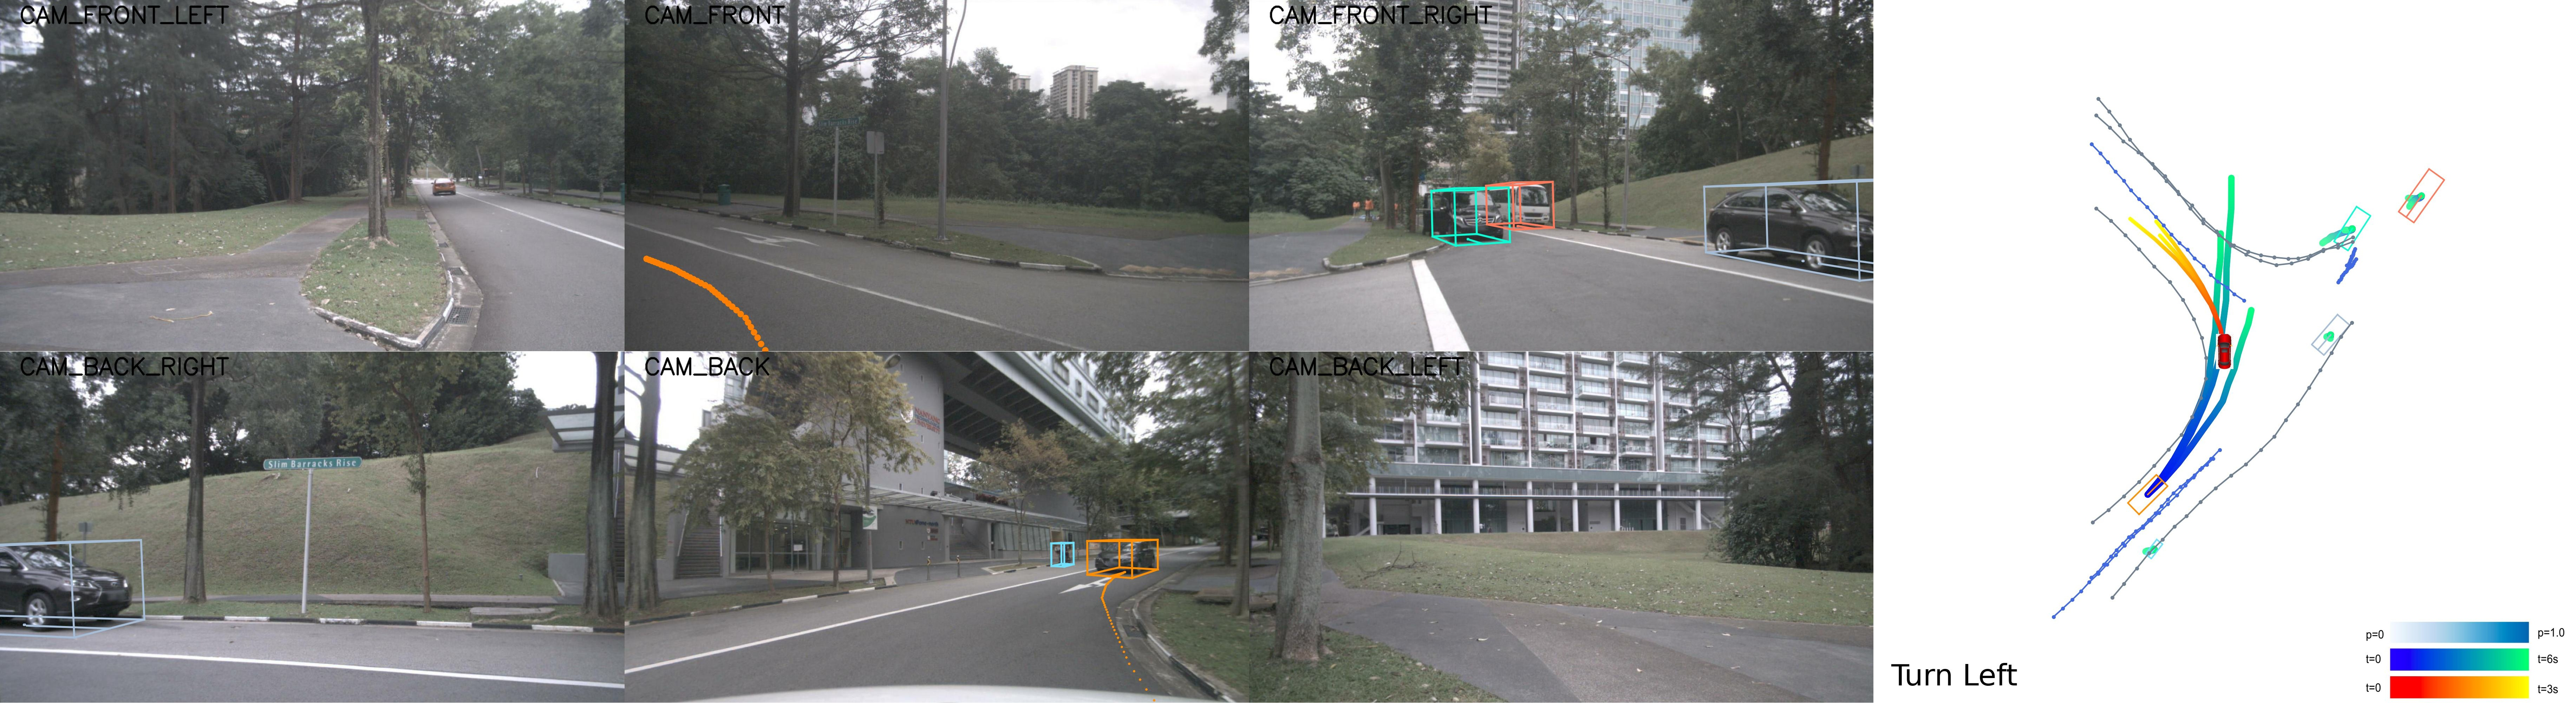
\includegraphics[width=1.0\linewidth]{Figures/vis/turn1.jpg}
  \end{subfigure}
  \begin{subfigure}{0.8\linewidth}
  \centering
  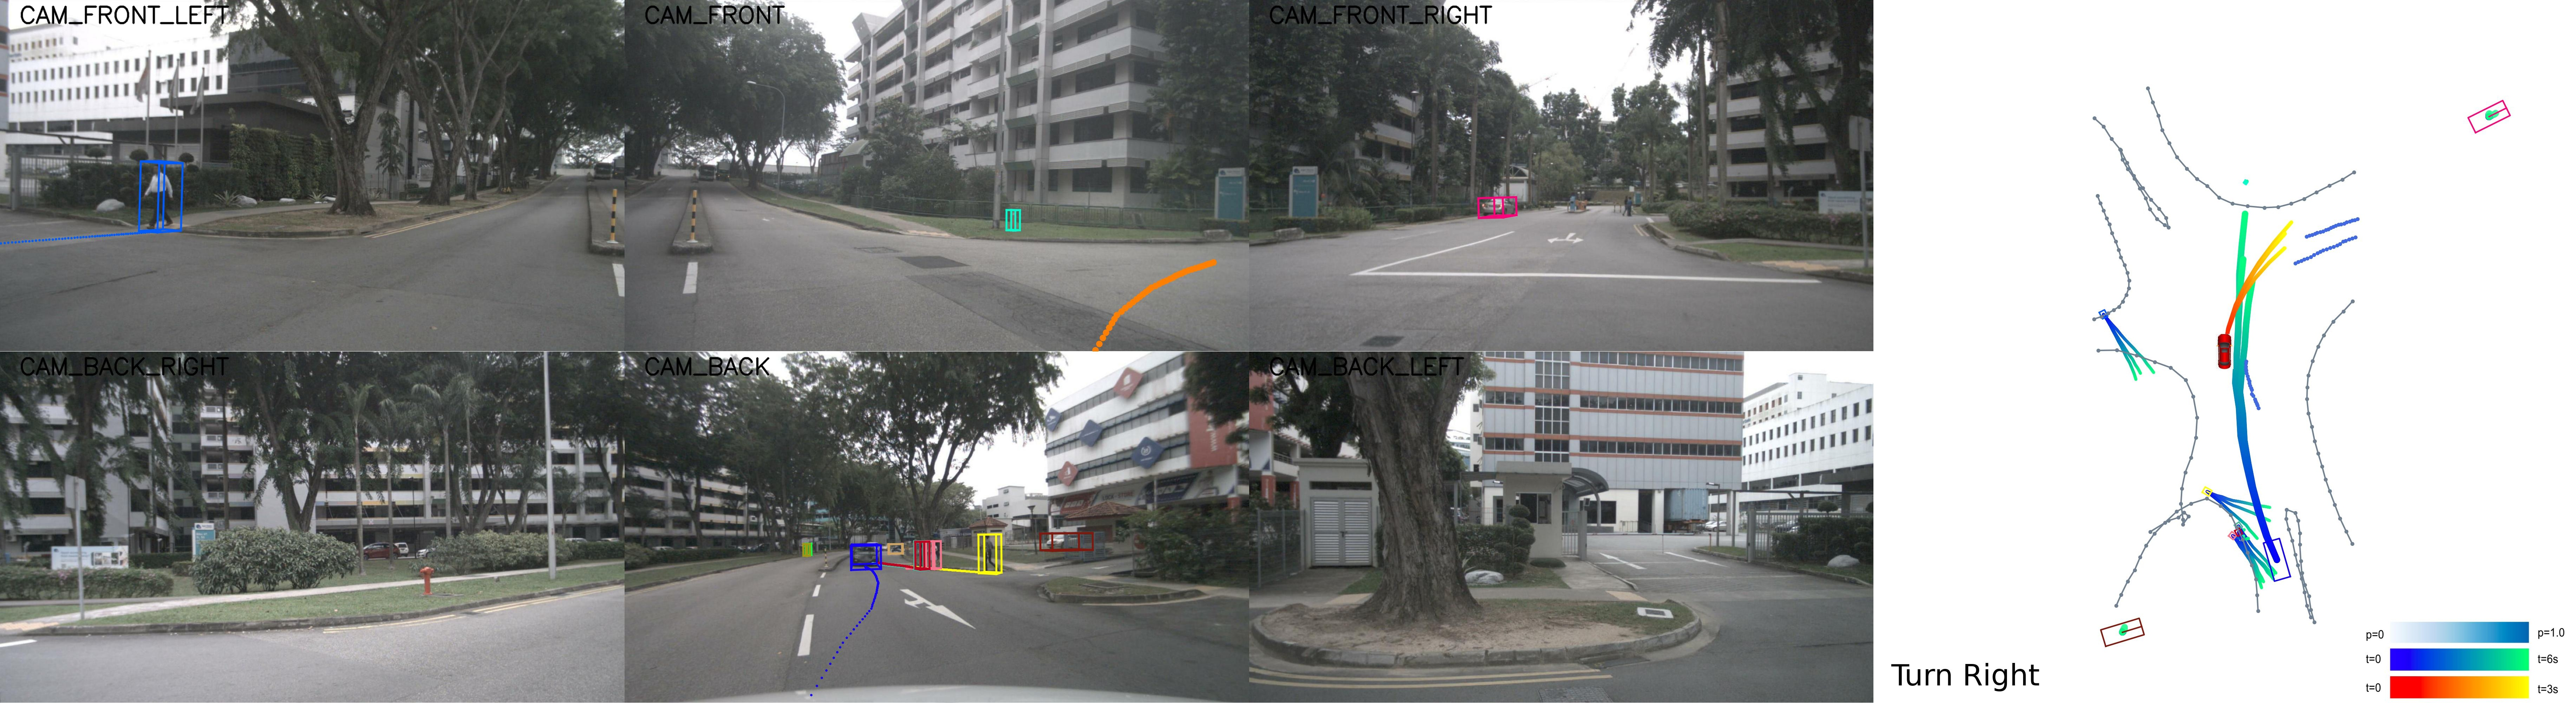
\includegraphics[width=1.0\linewidth]{Figures/vis/turn2.jpg}
  \end{subfigure}
  \begin{subfigure}{0.8\linewidth}
  \centering
  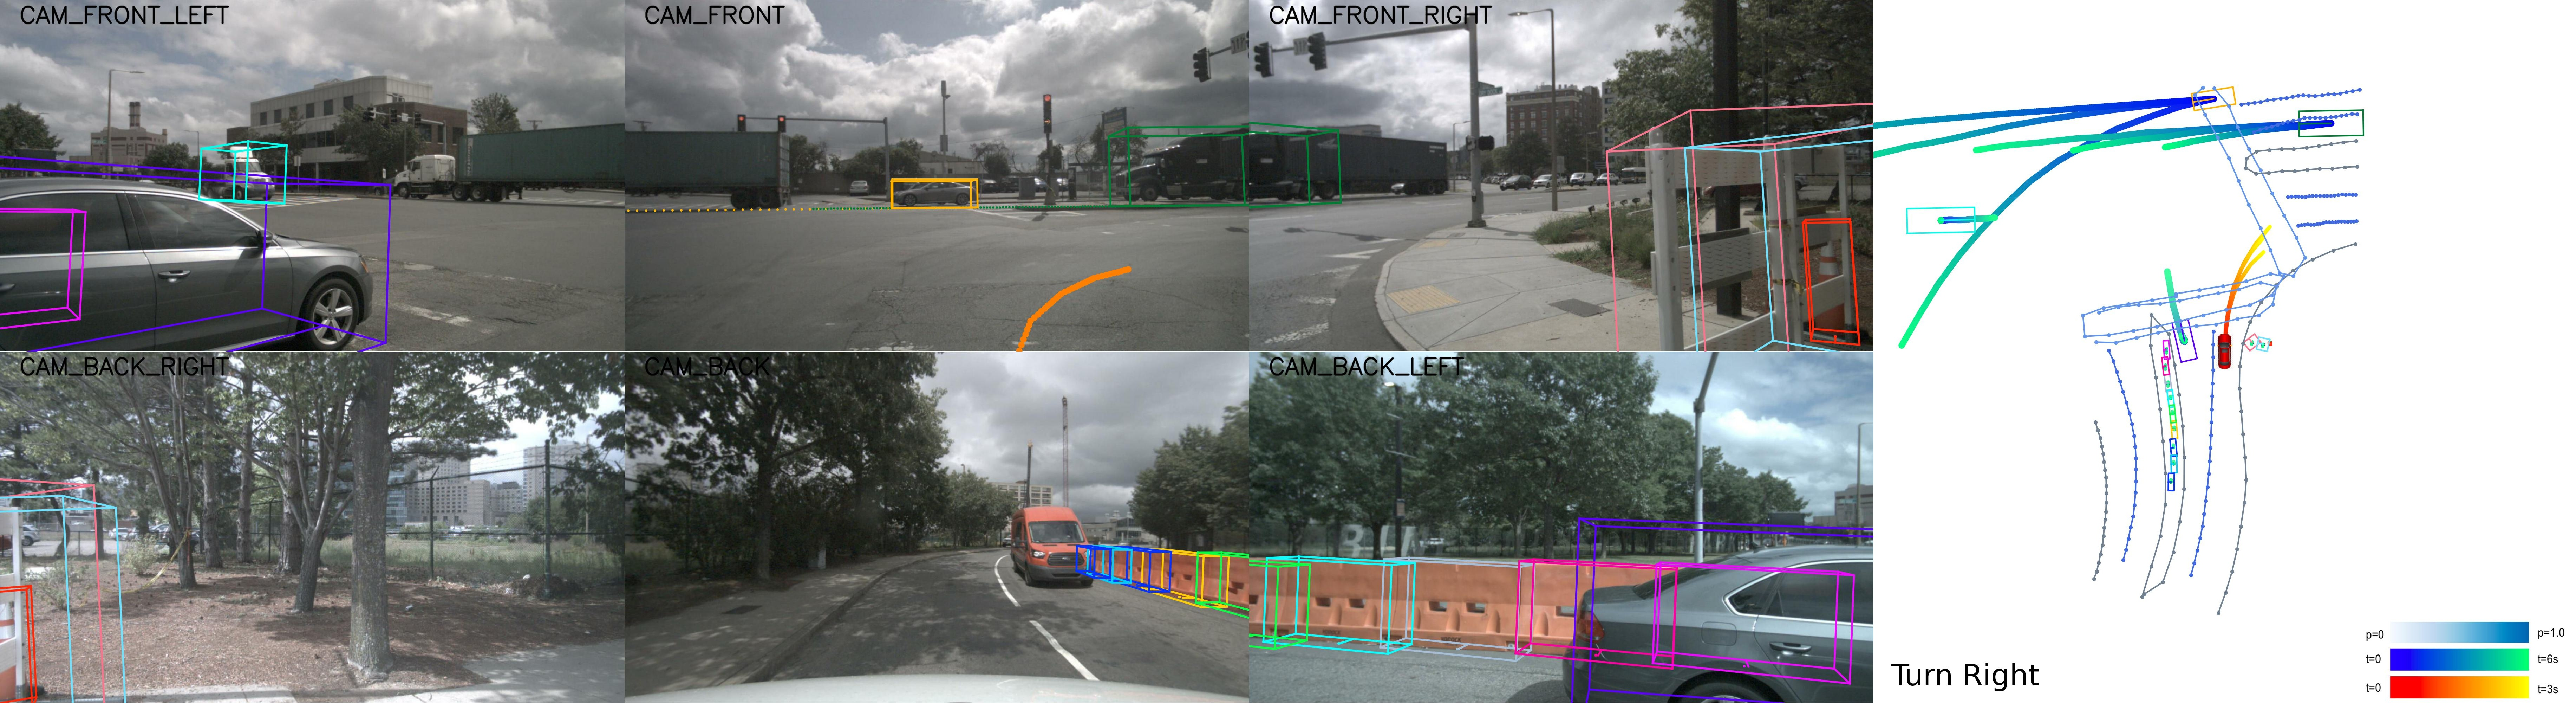
\includegraphics[width=1.0\linewidth]{Figures/vis/turn3.jpg}
  \end{subfigure}
  \begin{subfigure}{0.8\linewidth}
  \centering
  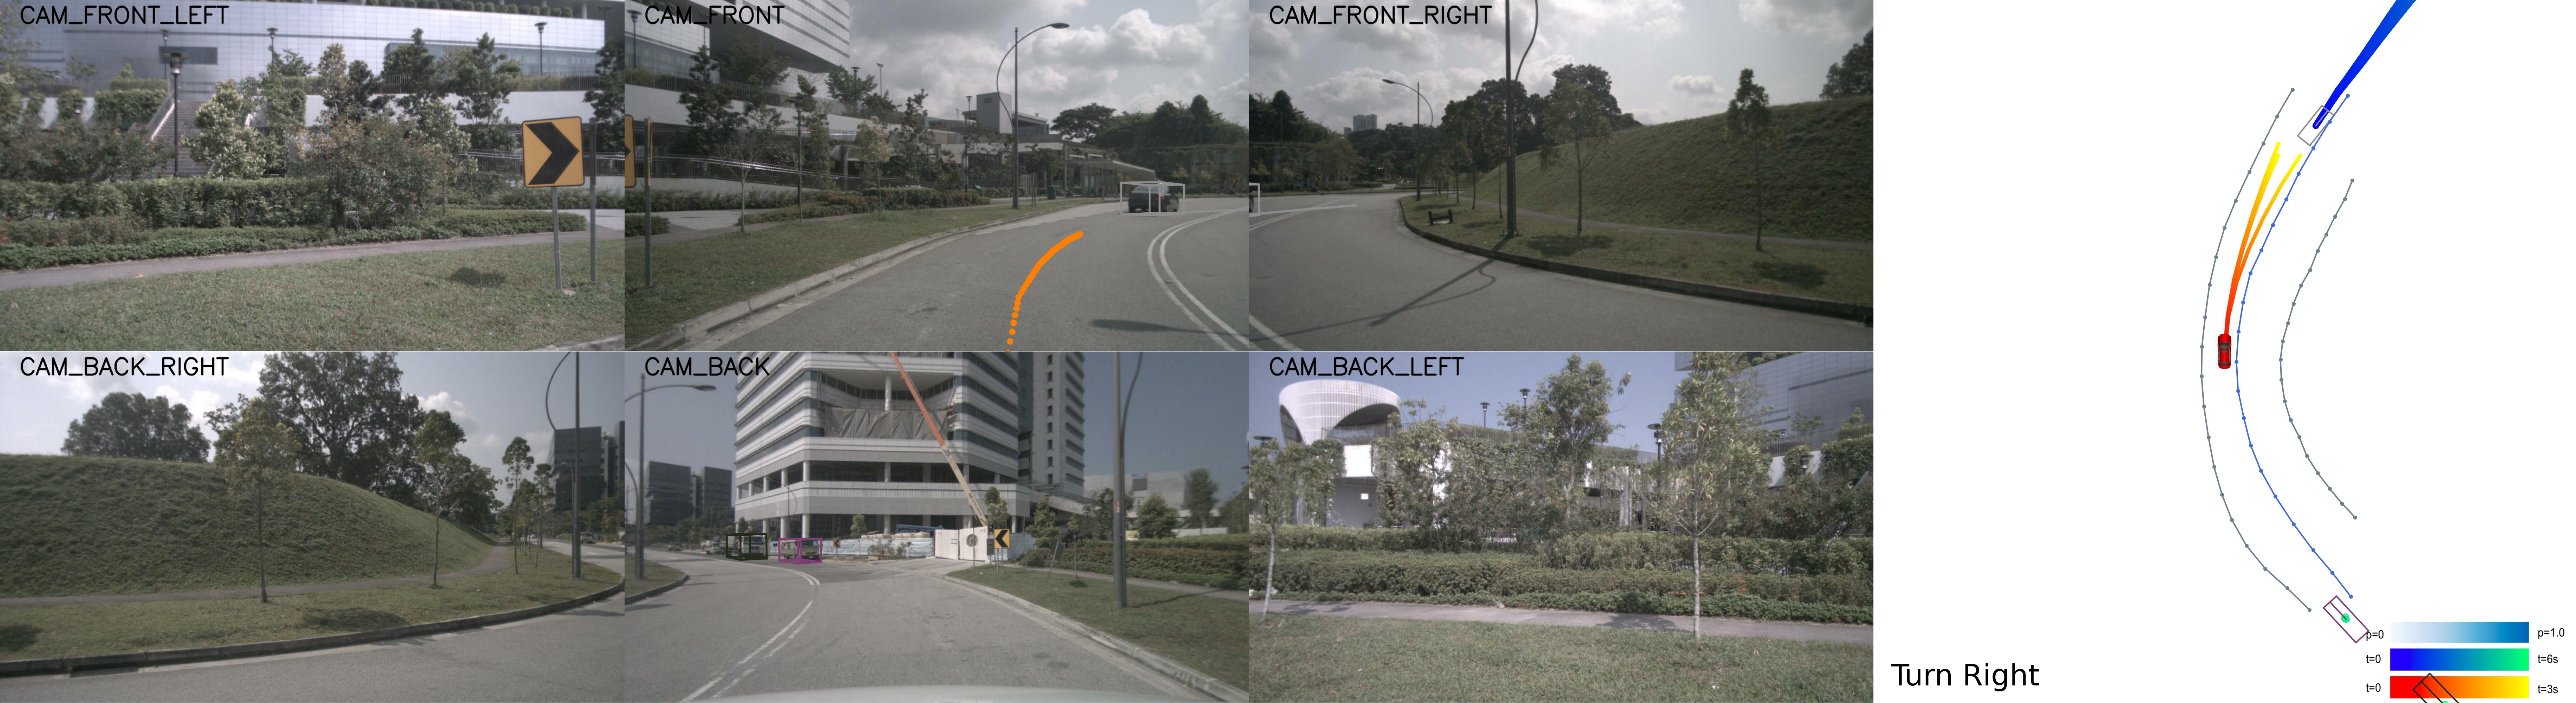
\includegraphics[width=1.0\linewidth]{Figures/vis/turn4.jpg}
  \end{subfigure}
  \caption{Visualization results. SparseDrive learnes different turning modes at intersections.}
  \label{fig:vis}
\end{figure}
\begin{figure}[htbp]
  \centering
  \begin{subfigure}{0.8\linewidth}
  \centering
  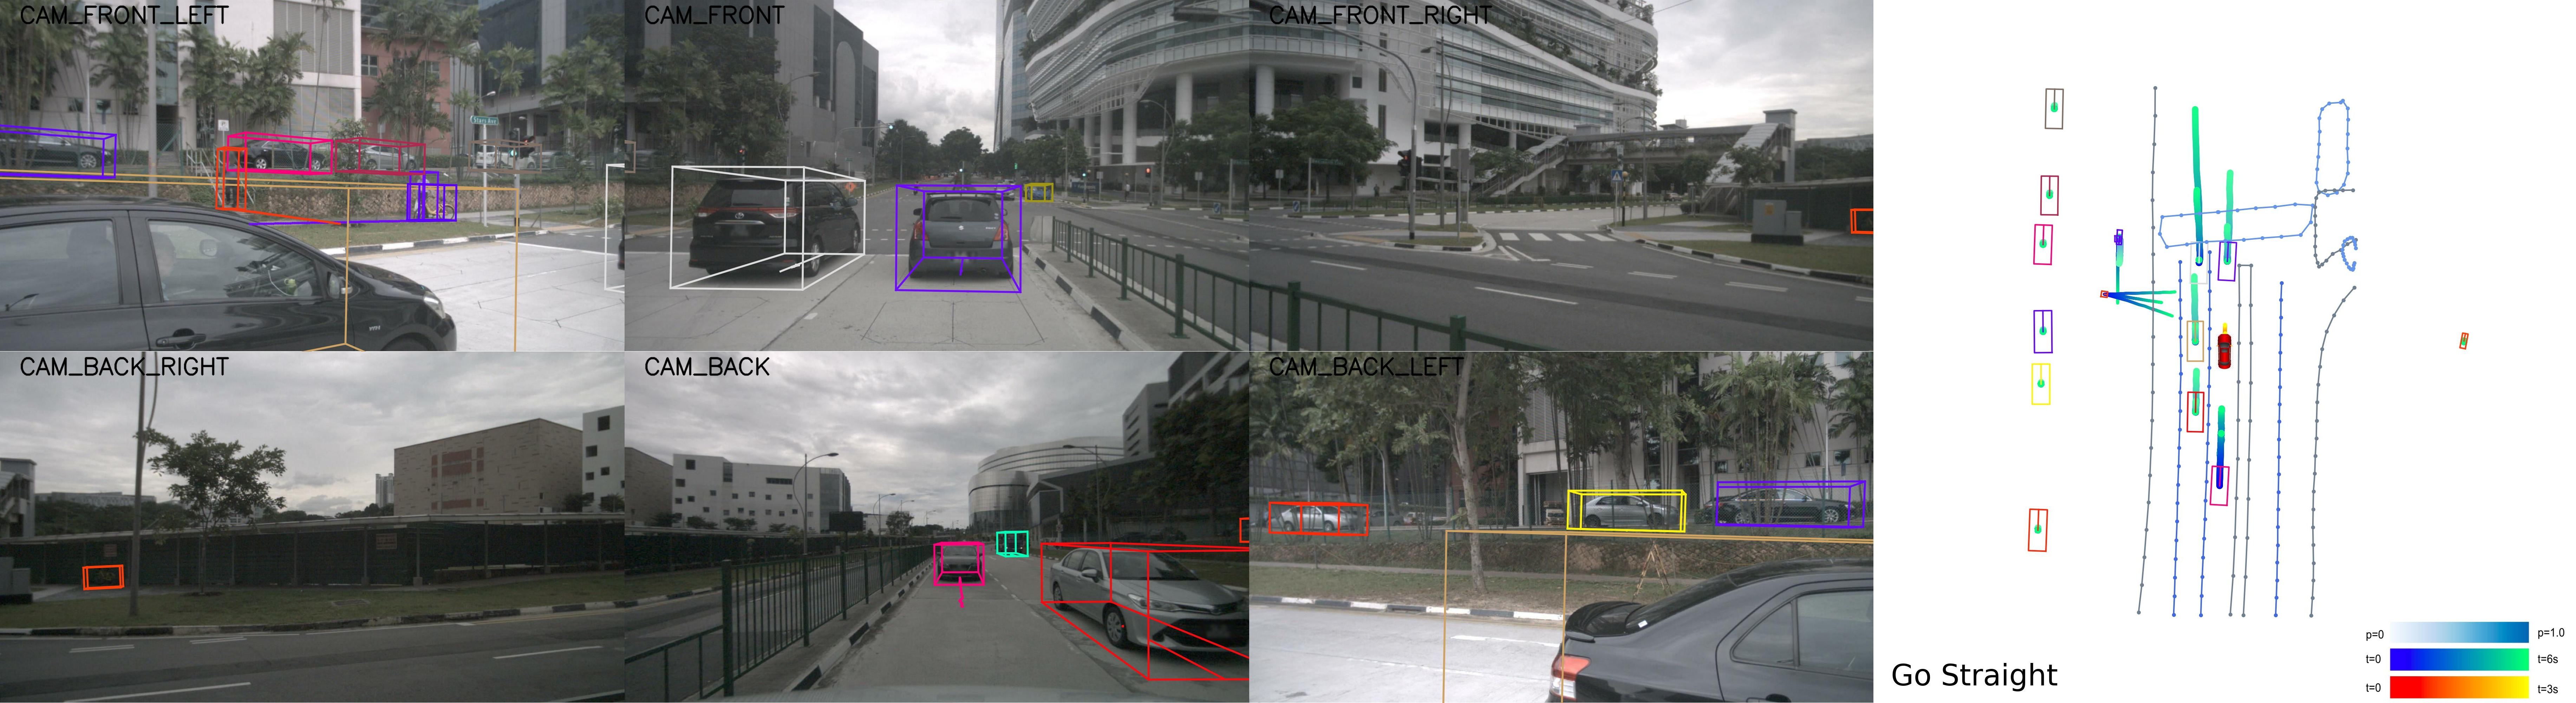
\includegraphics[width=1.0\linewidth]{Figures/vis/yield1.jpg}
  \end{subfigure}
  \begin{subfigure}{0.8\linewidth}
  \centering
  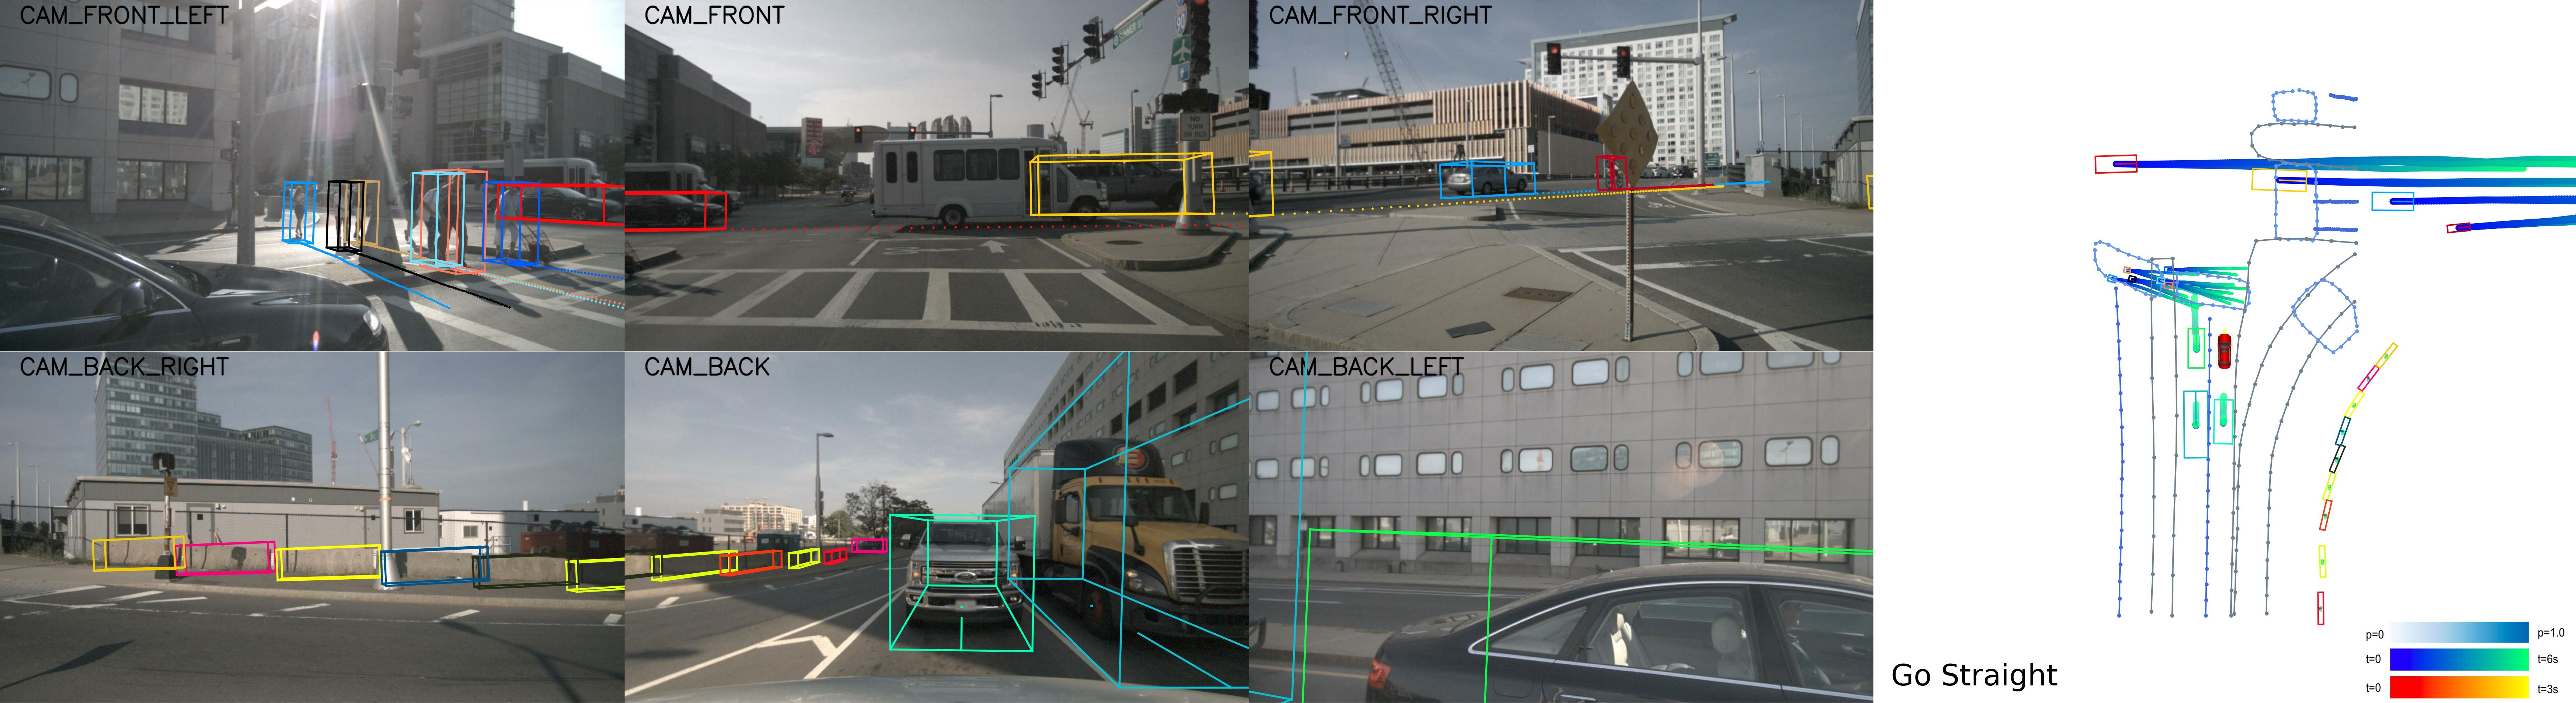
\includegraphics[width=1.0\linewidth]{Figures/vis/yield2.jpg}
  \end{subfigure}
  \begin{subfigure}{0.8\linewidth}
  \centering
  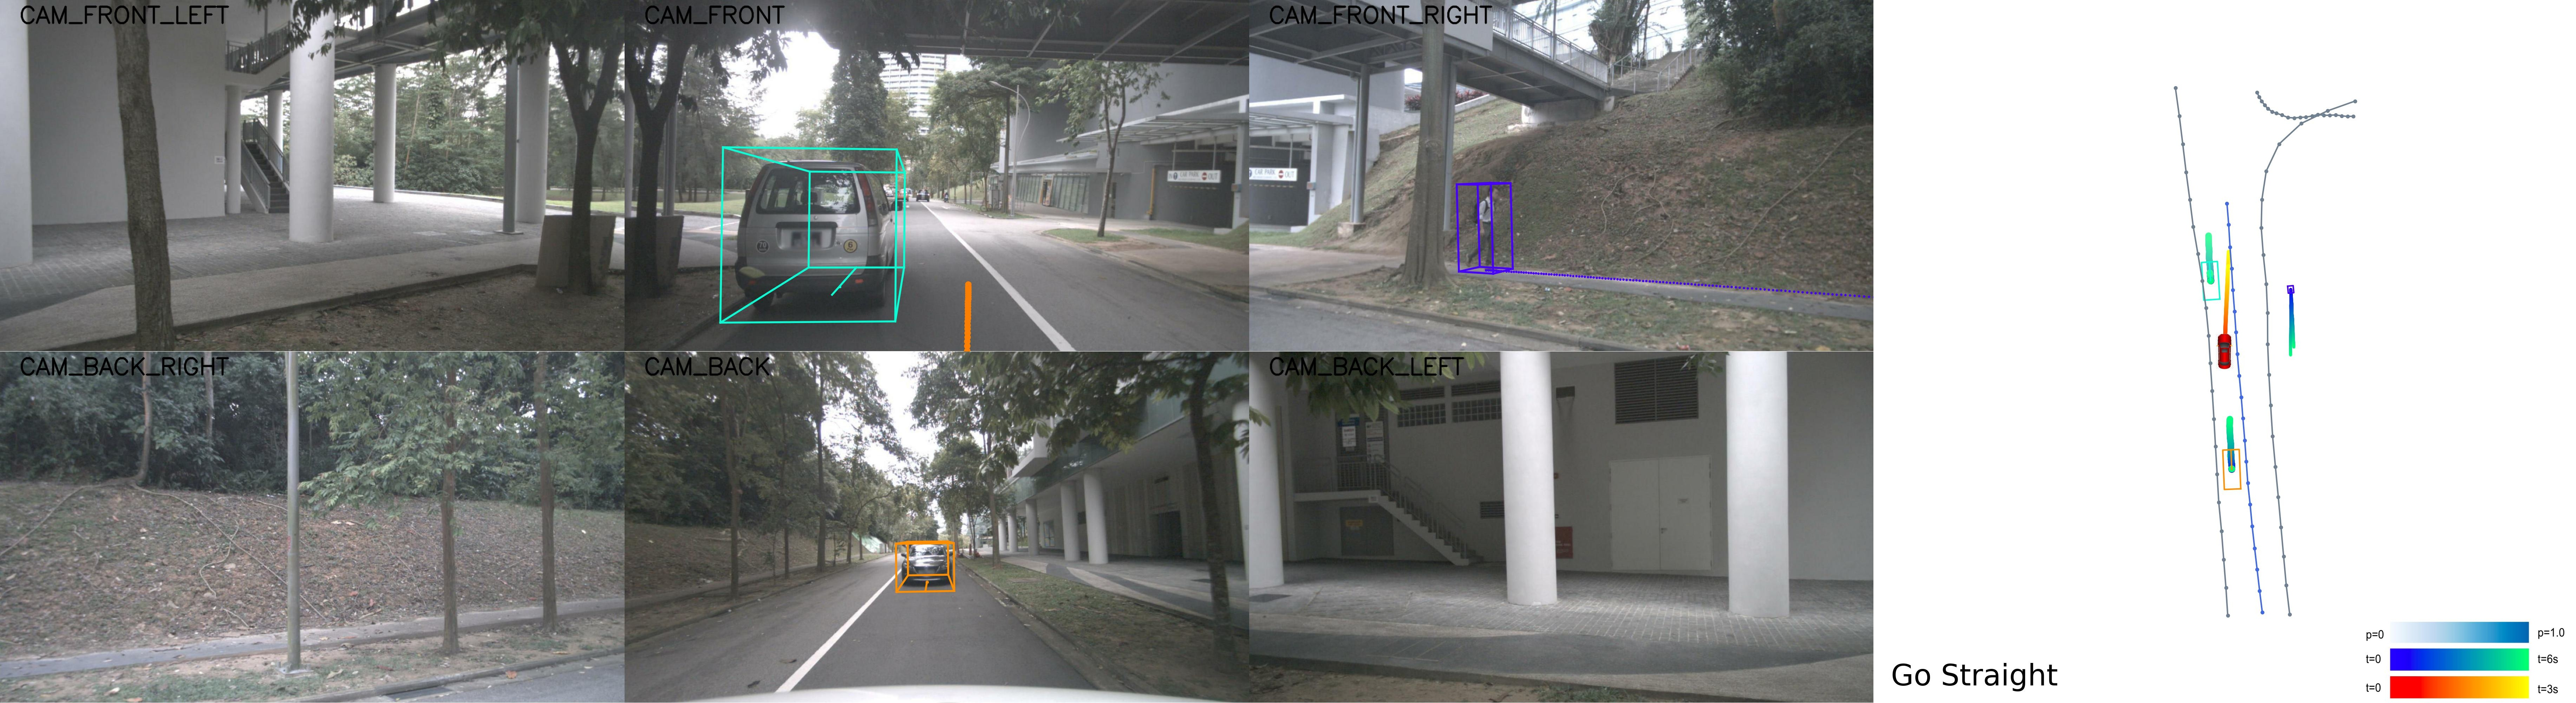
\includegraphics[width=1.0\linewidth]{Figures/vis/avoidance1.jpg}
  \end{subfigure}
  \begin{subfigure}{0.8\linewidth}
  \centering
  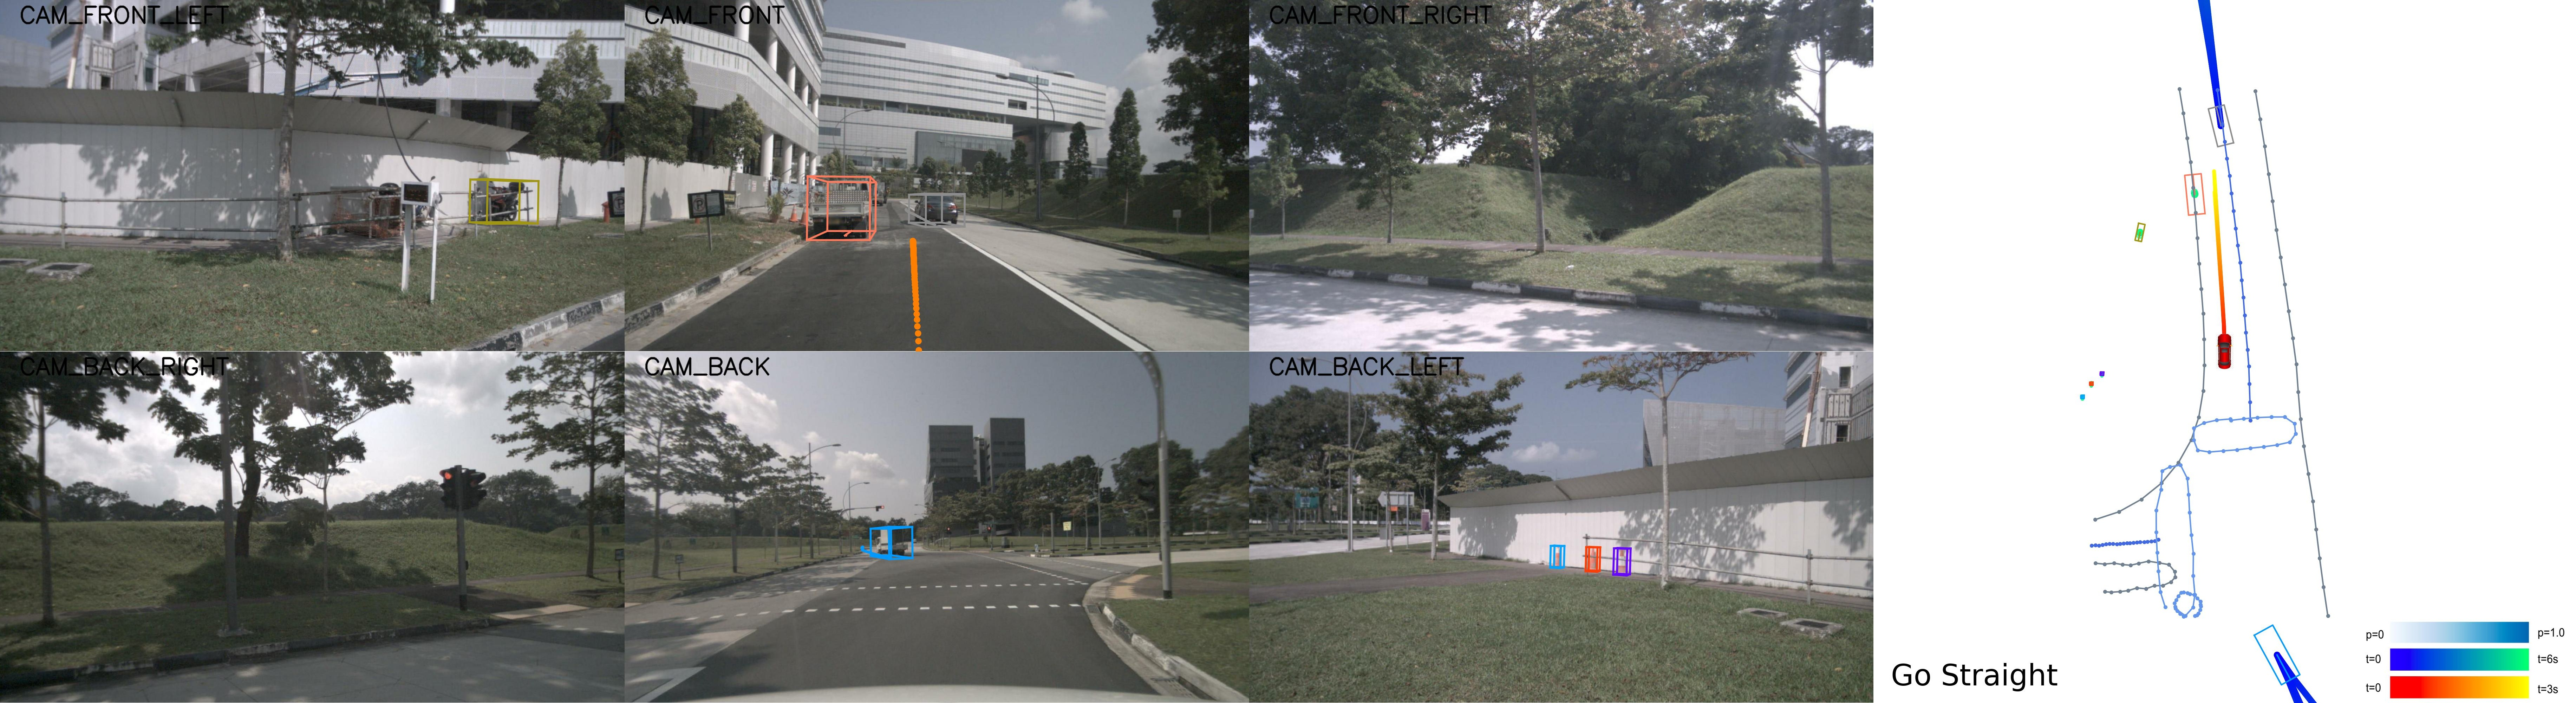
\includegraphics[width=1.0\linewidth]{Figures/vis/avoidance2.jpg}
  \end{subfigure}
  \caption{Visualization results. SparseDrive learns to yield to moving agents or avoid collision with obstacles.}
  \label{fig:vis}
\end{figure}